\documentclass[twocolumn,aps,prl,amsmath,amssymb,longbibliography]{revtex4-2}
\usepackage{graphicx}
\usepackage{dcolumn}
\usepackage{bm}
\usepackage{amsfonts}
\usepackage{xcolor,tabu}
\usepackage{multirow}
\usepackage{amsthm}
\usepackage{textcomp}
\usepackage{tikz}
\usepackage[colorlinks=true,
            linkcolor=blue,
            urlcolor=blue,
            citecolor=blue]{hyperref}
\hypersetup{bookmarksopen=true}
\usepackage{xr}
\externaldocument{correlation_SI}


\begin{document}
\title{Giant Number Fluctuations and Energy Spectra in 3-D Bacterial Turbulence}

\author{Zhengyang Liu}
%\email{liux3141@umn.edu}
\author{Wei Zeng}
\author{Xiaolei Ma}
\author{Xiang Cheng}


\affiliation{Department of Chemical Engineering and Materials Science, University of Minnesota, Minneapolis, Minnesota 55455, USA}

\date{\today}


\begin{abstract}
Giant number fluctuations, a landmark of collectively moving active particles, is universal in active systems across multiple length scales. Here, we present the first experimental study on the giant number fluctuation in 3-dimensional bacterial suspensions. Our measurements show that the number fluctuation scaled by the square root of mean number $\Delta N / \sqrt N$ scales with $N^{0.32}$ at high concentrations, confirming the theoretical predictions. Near the phase boundary, we observe a simultaneous increase of the scaling exponent and the flow induced by bacterial motions, suggesting a strong interplay between giant number fluctuations and flow. We show that this interplay spans all length scales in an active turbulence, by analyzing the kinetic energy spectra.

\end{abstract}

\maketitle

Giant number fluctuations (GNF), formally defined as the anomalously strong dependence of the variance of the number of particles on the mean number, is a universal phenomenon in active systems across multiple length scales, ranging from birds, fish and driven granules to bacteria, biological macromolecules and active synthetic particles \cite{Narayan2007, Aranson2008, Ward2008, Ballerini2008, Sokolov2009, Deseigne2010, Zhang2010,
Palacci2013, Schaller2013, Nishiguchi2017, Kawaguchi2017, Karani2019}. Predicted by the seminal works from Toner and Tu
\cite{Toner1995, Tu1998, Toner1998}, this phenomenon has stimulated extensive research interest and has become a landmark of ordered collectively moving particles
\cite{Toner2005, Ramaswamy2010, Vicsek2012, Saintillan2013, Marchetti2013}.

Over the last 20 years, the understanding of GNF has been deepened significantly. Despite the progress, two important questions are still awaiting definite answers.
First, the exact value of the scaling exponent of the variance on the mean has not reached an agreement. While the GNF is a seemingly universal in many systems, the scaling exponents measured or calculated in different systems show remarkable discrepancy \cite{AditiSimha2002, Ramaswamy2003, Narayan2007, Chate2008, Deseigne2010, Zhang2010,
Dey2012, Saintillan2012, Schaller2013, Ngo2014, Nishiguchi2017, Kawaguchi2017, Mahault2019,
Karani2019}. In particular, the experimental works so far have reported scaling exponent ranging from 0.13 to 0.5 (the scaling exponent $\alpha$ is defined as $\Delta N /\sqrt N \propto N^\alpha$, $\Delta N$ is the standard deviation of particle number and $N$ is the mean number)
\cite{Narayan2007, Deseigne2010, Zhang2010, Schaller2013, Nishiguchi2017, Kawaguchi2017, Karani2019}, making it hard to compare experimental results with theory and simulations. We understand this situation by realizing that all the experiments have been done in 2-dimensional systems, with one or more frictional walls in direct contact to the active particles. We also notice that, although several experimental studies on bacterial systems have been reported, the GNF in bacterial turbulence - arguably the most fascinating and striking manifestation of microswimmer collective motions - has not been investigated (Supplementary movie 1 shows a vigorous bacterial turbulence in motion). Second, the driving force of GNF remains largely unclear. Although mechanisms based on nematic instability
\cite{AditiSimha2002, Ramaswamy2003, Narayan2007} and topological defects \cite{Saintillan2008b, Schaller2013} have been proposed or observed in specific systems, the driving force of GNF in other active systems, especially 3-dimensional systems dominated by hydrodynamic effects, remains unknown.

% We hope this result deepens the current understanding of GNF in bacterial active turbulence, and will eventually lead to a theory that quantitatively captures experimental results.

In this letter, we present an experimental measurement of GNF in 3-dimensional bacterial turbulence. Due to the absence of frictional walls, our results can provide a solid benchmark for other works to compare to. Meanwhile, our 3-D GNF measurement enables deeper studies on this universal phenomenon, such as the dimensionality effect. We also present a systematic measurement on the flow fields in active turbulence using particle image velocimetry (PIV), which has been shown to be a powerful tool in studying turbulent flows, and has been adopted to study active turbulence recently
\cite{Ishikawa2011, Wensink2012, Sokolov2012, Sanchez2012, Dunkel2013, Schaller2013, Peng2020}. Fig.~\ref{fig:1}d-e show the flow fields obtained from PIV analysis in dilute (1.6\%) and dense (6.4\%) bacterial suspensions. A detailed analysis on the velocity fields reveals a strong correlation between flow strength and GNF at multiple length scales.

Counting particle numbers poses a major challenge in measuring the GNF of 3-dimensional bacterial turbulence. Looking at the bright field microscopy images of a dense 3-dimensional bacterial suspension (Fig.~\ref{fig:1}c, and Supplementary movie 1), one immediately realizes that it is not possible to directly count the number of bacteria. Fortunately, the spatial distribution of bacterial concentrations can be inferred from optical microscopy images, where dark region indicates high local concentration and bright region indicates low local concentration. This idea is an extension of Beer-Lambert law which correlates solution concentration with its light attenuation. Similar principle has been used in some inspiring experimental works using image intensity as local concentration indicators \cite{Wilson2011, Schaller2013}. To be more quantitative on the relation between concentration and image pixel intensity, we did a calibration experiment by preparing bacterial suspensions of volume fractions ranging from 1.6\% to 7.2\% and take images of them under the same illumination. The images corresponding to different volume fractions are shown in Fig.~\ref{fig:1}a. As expected, when volume fraction gets higher, the image becomes dimmer. We plot the volume fractions as a function of the mean pixel intensities in the corresponding images, and find that the relation is almost linear, as shown in Fig.~\ref{fig:1}b.


\begin{figure}[h]
\begin{center}
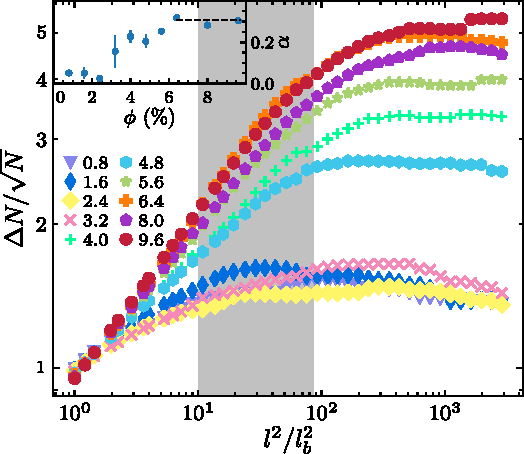
\includegraphics[width=0.45\textwidth]{figures/fig-1/v3.pdf}
\caption[Experimental details]
{
(a) Bacterial suspensions of different volume fractions under the same illumination conditions.
(b) Volume fraction as a function of averaged pixel intensities.
(c) Bacterial active turbulence displaying constantly varying concentration inhomogeneity (6.4\%). Scale bar is 100 \textmu m.
(d), (e) Velocity field of a dilute bacterial suspension (1.6\%) and (6.4\%). Scale bars are 135 \textmu m.
}
\label{fig:1}
\end{center}
\end{figure}


% Bacterial suspensions are premier example of active matter. Being constantly driven out of equilibrium, they exhibit anomalous properties drastically different from systems in equilibium, including enhanced diffusivity, reduced viscosity and giant number fluctuations. While the anomalous diffusion and rheology have only been demonstrated in microscopic scale, the giant number fluctuations are found to be more universal across multiple length scales. Indeed, such fluctuations have been observed in bird flocks \cite{Ballerini1232}, fish schools \cite{Ward6948}, shaking granules \cite{Narayan105}, bacteria on agar gels \cite{Zhang13626} and active actin filaments \cite{Schaller4488}. \textcolor{red}{Though the phenomenon appears to be universal, the underlying mechanisms can be different. citation needed}
%
% Despite the extensive efforts to model and measure giant number fluctuations in a variety of systems, there still lacks detailed and systematic measurements, leaving the mechanism of the phenomenon unclear. First, how the fluctuation depends on the crowdedness of "swimmers" is not elucidated. Although it has been shown that the fluctuation is stronger in crowded environment \cite{PhysRevE.95.020601, Zhang13626}, most experiments to date have assumed two regimes: low concentration and high concentration. Within each concentration regime, fluctuations are identical. In other words, at high concentrations, number fluctuations are always of the same magnitude, while at low concentration, giant number fluctuations become absent. The simple picture was great for appreciating the macroscopic concsequences of collective motions. However, a lack of detailed measurements on concentration dependence hindered the discovery of the microscopic origin of giant number fluctuations. The subtle dependence of number fluctuations on concentration has been hinted by experiment with bacteria on 2-D surface\cite{Zhang13626}. In this paper, we present a more systematic measurement on concentration dependence. The results reveal the microscopic origin of giant number fluctuations. Second, how the magnitude of giant number fluctuation evolves has never been measured, which is due to the fact that the most widely used experimental platform - bacterial suspensions - suffers from a lack of control over the motility of bacteria. We overcome this limitation by engineering a light-controlled \textit{E. coli} strain, whose primary energy source is light. The swimming speed of such strain can be instantaneously and precisely controlled. This evolution can reveal the intrinsic time scale of an active system. More importantly, comparisons can be made with the evolution of other quantities \cite{Peng2020}, such as flow order and flow energy, to reveal the underlying mechanisms of giant number fluctuations. Third, while theories predict that giant number fluctuations depend on dimensionality \cite{PhysRevLett.75.4326, PhysRevE.58.4828, EPL2003, doi:10.1146/annurev-conmatphys-031119-050752}, all simulations and experiments so far have been done in 2-dimensional space
% \cite{PhysRevE.77.046113, PhysRevLett.123.218001, Schaller4488, PhysRevE.95.020601}. We examine giant number fluctuations in 3-D space experimentally for the first time, and also compare the result with 2-D space under similar experimental settings. These measurements will enable us to understand the theoretical predictions, and will provide a good platform for testing and developing existing theories.
%
% \begin{figure}[h]
% \begin{center}
% 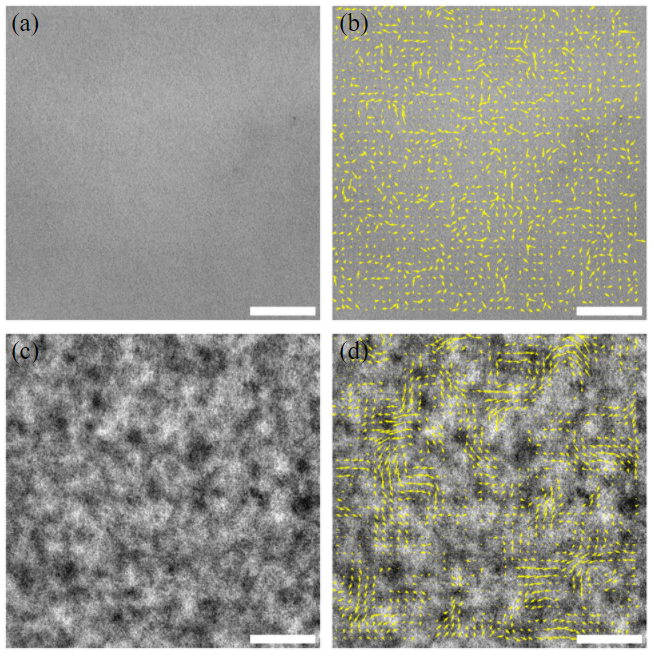
\includegraphics[width=0.45\textwidth]{figures/fig-1-v2.png}
% \caption[]{Bright-field microscopy of a bacterial suspension at 20 n$_0$ and 80 n$_0$ (a, c) and the corresponding velocity fields(b, d). Scale bars are 100 \textmu m.}
% \label{fig:1}
% \end{center}
% \end{figure}
%
% Measuring instantaneous local bacterial concentration is the key to quantify the magnitude of giant number fluctuations. Yet, it is challenging. Inspired by earlier experimental works, where fluorescence intensity serve as indicators of local concentration \cite{Schaller4488}, we come up with the idea that light transmission - the natural information in bright field microscope images - could also serve as local concentration indicators. This idea is an extension of Beer-Lampert law, where the attenuation of light and particle concentration are related. Such principle is used in spectrophotometer, with which we measure the concentration of our bacterial suspensions. Similar idea, where fluctuations in image intensity is proportional to fluctuations in concentration ($\Delta I=\kappa\Delta\rho$), was assumed in another work \cite{PhysRevLett.106.018101}. Here, we experimentally verify the assumption, showing that concentration and image intensity follow a nearly linear relationship (\textcolor{red}{Fig.~S1}). The idea is illustrated in Fig.~\ref{fig:1}c - a snapshot of dense bacterial suspensions - where giant number fluctuations lead to strong alternation of dark and bright regions, which correspond to high concentration regions and low concentration regions, respectively. In contrast, in a dilute suspension shown in Fig.~\ref{fig:1}a, where giant number fluctuations are absent, such intensity alternation is not observed.
%
% Since local concentration measurement is made possible by the idea of using image intensity as a concentration indicator, we are able to fill in the missing pieces in the knowledge of giant number fluctuations in 3-D bacterial suspensions. Our most important finding is that: motility induced fluid flow drives the giant number fluctuations and determines the magnitude of number fluctuations. We also show that fluid convection is the microscopic origin of local number fluctuations, in consistency with then main finding. Moreover, we show that in a confined quasi-2D geometry, giant number fluctuation gets weaker, which again confirms the key finding, since motility induced flow is largely suppressed due to the closely spaced no-slip boundaries. This work presents systematic measurements on giant number fluctuation, providing a good platform for testing and developing active matter theories. By relating microscopic dynamics and macroscopic properties, our findings shed new light on the mechanisms of emergent collective behaviors in active matter.
%
%
% \begin{figure}[!]
% \begin{center}
% 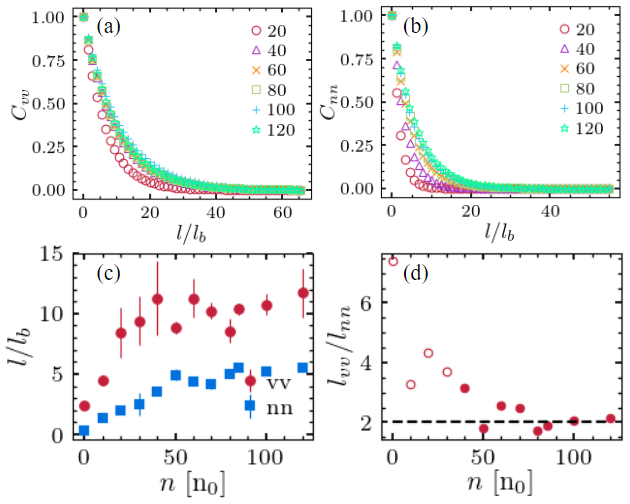
\includegraphics[width=0.45\textwidth]{figures/fig-2-v2.PNG}
% \caption[]{\textbf{Spatial correlation functions and correlation lengths.} (a, b) velocity and image intensity correlation functions, (c) velocity and image intensity correlation length (defined as $C=1/e$) and (d) ratios between the two correlation lengths at concentrations = 20, 40, 60, 80, 100 and 120 n$_0$.}
% \label{fig:2}
% \end{center}
% \end{figure}
%
% \textit{Spatial correlations}--We analyzed the spatial correlations of flow velocity and concentration (Fig.~\ref{fig:2}a-b) of motile \textit{E. coli} suspensions at various concentrations. Both correlation lengths show a gradual increase at low concentration and saturate at high concentration (Fig.~\ref{fig:2}c). The crossover concentration of both correlation lengths are around 40-50 n$_0$, suggesting a transition from a disordered state to turbulence. The gradual increase at low concentration suggests that, even below the apparent turbulent transition, bacteria, or more generally active agents, start to move in a correlated way \cite{PhysRevLett.119.028005}. \textcolor{red}{Remarkably, we show that above the crossover concentration, the ratio between velocity correlation length and concentration correlation length converges to 2 (Fig.~\ref{fig:2}d). We have not fully understood the significance of this ratio, but it tends to suggest a close correlation between concentration and velocity field. In the following analysis of giant number fluctuations, we hope to elucidate this correlation.} Moreover, our finding suggest that spatial concentration correlation length, in addition to flow velocity correlation length\cite{Wensink14308, PhysRevLett.110.228102}, can be used to mark the transition to active turbulence.
%
% \begin{figure*}[!]
% \begin{center}
% 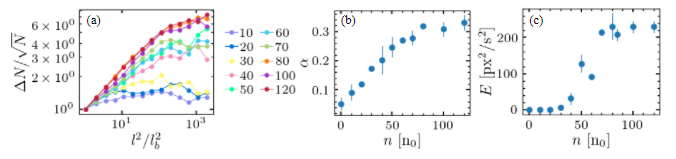
\includegraphics[width=\textwidth]{figures/fig-3-v3.png}
% \caption[]{\textbf{Concentration dependence} (a) Giant number fluctuations in bacterial suspensions at concentrations ranging from 10 to 120 n$_0$. The $\Delta N/\sqrt{N}$ is in fact $\Delta I/l$, where $I$ is the average pixel intensity of a subsystem and $l$ is the linear size of the subsystem. The $\Delta N/\sqrt{N}$ value is rescaled by the first value of each curve, so that all the curves start from $\Delta I/l=1$. (b) The scaling exponents $\alpha$ ($\Delta N \propto N^{0.5+\alpha}$) of number fluctuation curves as a function of bacterial concentrations. (c) Steady- state flow energy as a funciton of bacterial concentrations.}
% \label{fig:3}
% \end{center}
% \end{figure*}
% \textit{Concentration dependence--}We measured the number fluctuations at concentrations ranging from 10 n$_0$ to 100 n$_0$. As can be seen in Fig.~\ref{fig:3}a, as concentration gets higher, the fluctuation gets stronger and deviates farther from thermal equilirium. A more quantitative description of the concentration dependence is shown in Fig.~\ref{fig:3}b, where the scaling exponents $\alpha$ extracted from Fig.~\ref{fig:3}a are plotted against concentrations. $\alpha$ gradually increases with concentrations, and plateaus above 70 n$_0$. The plateau value of $\alpha$ at high concentrations is around 0.32, close to the theoretical prediction made by Simha and Ramaswamy \cite{PhysRevLett.89.058101}. Their theory follows from a set of hydrodynamic equations of motion, and implies that the standard deviation $\Delta N$, scaled by
% $\sqrt N$, diverges as $N^{1/3}$. At low concentrations, $\alpha$ increases smoothly up to 70 n$_0$, different from the turbulence transition, 40-50 n$_0$, marked by the crossover of velocity and concentration correlation lengths. This difference is defying our intuition that the giant number fluctuations are always the same once turbulent state is triggered. Such difference is attributed to flow energy. In Fig.~\ref{fig:3}c, we plot the steady-state flow energy, defined as the sum of velocity squares, as a function of concentration. This result suggests that, above 40 n$_0$, within the turbulent state, the steady-state flow energy is not constant. Instead, it shows an abrupt increase from 40 n$_0$ to 70 n$_0$, after which it plateaus. The range of flow energy increase coincides with the range of increasing of $\alpha$, implying a correlation between flow energy and magnitude of number fluctuations. This correlation will appear again and get more evident further on.
%
% \begin{figure}[ht]
% \begin{center}
% 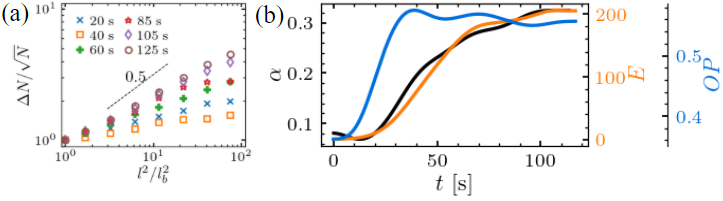
\includegraphics[width=0.5\textwidth]{figures/fig-4-v2.png}
% \caption[]{\textbf{Evolution of giant number fluctuations at concentration $n=80$ n$_0$.} (a) Standard deviation of particle numbers $\Delta N$ scaled by the square root of the mean $\sqrt N$ as a function of subsystem size rescaled by bacterial body size $l^2/l_b^2$. Numbers in legends denotes the time from the point when bacterial motility is triggered by light (seconds). (b) The temporal evolution of the scaling exponents $\alpha$, flow energy $E$ and flow order parameter $OP$.}
% \label{fig:4}
% \end{center}
% \end{figure}
%
% \textit{Evolution--}By virtue of the light-controlled \textit{E. coli}, we are able to image how a "dead" suspension gradually start to mix, form patterns, deviate from the thermal equilibrium and exhibit giant number fluctuations. Fig.~\ref{fig:4}a shows how standard deviation scales with the mean and how it evolves over time. Initially, the collective motion is not fully developed, and the scaling exponent $\alpha$ is low. After 100 seconds, the increase of $\alpha$ slows down. The evolution of $\alpha$ is shown in a finer temporal resolution in Fig.~\ref{fig:4}b. In addition, the flow energy and flow order parameter for the same process are plotted as well in Fig.~\ref{fig:4}b \cite{Peng2020}. High flow energy indicates that the fluid elements are moving vigorously, and high order parameter indicates that most of the flows are moving along the directions of their neighbors. When order parameter is high, the flow field appears to us as a turbulence. The order parameter initially increases, and then reaches a plateau value of 0.56 at 40 seconds. At this point, the flow already looks like turbulence, but the energy is still low. After another 60 seconds, flow energy also reaches a plateau and the flow is then exhibiting the most vigorous turbulence. Remarkably, we find that $\alpha$ and $E$ evolve almost along the same trajectory, and both reach a high plateau value at 100 seconds. This coincidence is again pointing to the correlation between flow energy and magnitude of number fluctuations.
%
% \begin{figure}[b]
% \begin{center}
% 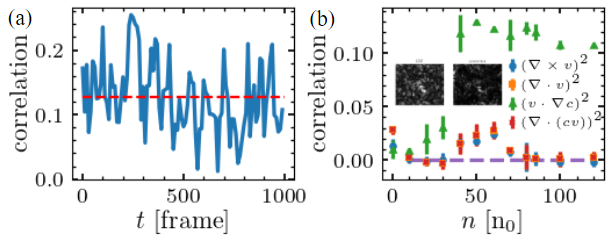
\includegraphics[width=0.5\textwidth]{figures/fig-5-v2.png}
% \caption[]{\textbf{Correlations of local concentration fluctuation with flow field.} (a) Time series of correlation between local concentration fluctuation and convection. (b) Correlations of local concentration fluctuation with vorticity, divergence, convection and divergence of concentration weighted velocity. Insets show a snapshot of local concentration fluctuation field and convection field in a 80 n$_0$ bacterial suspension at steady state.}
% \label{fig:5}
% \end{center}
% \end{figure}
%
% \textit{Microscopic origin--}To uncover the microscopic origin of the giant number fluctuations, we analyze the correlation between local concentration fluctuation and local flow field. The local concentration fluctuation is defined as the standard deviation of local concentration over a period of time, where the length of the time is determined by the autocorrelation time of concentration. The flow field has several meaningful derivatives, including the curl of velocity, the divergence of velocity, the divergence of concentration weighted velocity and velocity dotted into concentration gradient. These derivatives quantify the energy dissipation, topological defects, particle fluxes and particle convection, respectively. \textcolor{red}{The assumption here is that if the local fluctuation shows high correlation with one of the derivatives of the local flow field, this derivative is likely to be the driving force of the local concentration fluctuation, and thus the driving force of the global giant number fluctuations. Though it is possible that none of these flow field derivatives shows high correlation, our measurement on the concentration dependence and the evolution, as well as other existing works \cite{PhysRevLett.100.178103, Schaller4488} all suggest that the flow field plays a key role in giant number fluctuations.} Fig.~\ref{fig:5} shows the correlations between local concentration fluctuation and various flow field derivatives. The correlations are between two fields are computed as described in (\textcolor{red}{SI: Method}). These correlations usually fluctuate, and sometimes the amplitude can be quite large, as shown in Fig.~\ref{fig:5}a. Nonetheless, the mean correlation over a long time can still reflect the relationship between two fields. For perfectly correlated fields, the correlation can be as much as one. For uncorrelated fields, however, the mean over thousands of frames can always make the correlation vanish.
% Fig.~\ref{fig:5}b shows the correlations at concentrations ranging from 10 to 120 n$_0$.
% Among all the flow field derivatives, the convection, $v\cdot\nabla c$, shows the highest correlation with local concentration fluctuation. In addition, the correlation shows a similar trend as that of the velocity and concentration spatial correlation lengths, where a plateau is found above 40 n$_0$. These observations suggest that the convection is the microscopic origin of local conconcentration fluctuation, and is also the leading cause of the giant number fluctuations in dense bacterial suspensions.
%
% \begin{figure}[!]
% \begin{center}
% 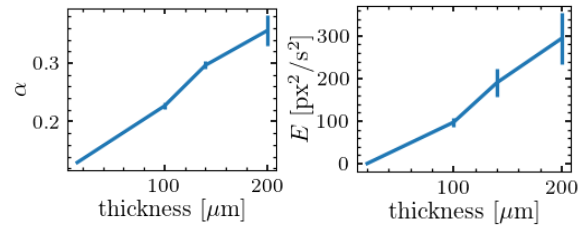
\includegraphics[width=0.5\textwidth]{figures/fig-6-v1.png}
% \caption[]{Giant number fluctuations magnitudes (a) and flow energy (b) at gap thicknesses 20, 100, 140 and 200 \textmu m ($n=85$ n$_0$).}
% \label{fig:6}
% \end{center}
% \end{figure}
%
% \textit{Dimensionality effect--}\textcolor{red}{The dimensionality effect is also investigated by gradually reducing the gap size from the bulk limit 200 \textmu m down to 20 \textmu m, a quasi-2D geometry, by using thinner coverslips as the spacer between the top and bottom glass slides. $\alpha$, the magnitude of giant number fluctuations, is found to decrease monotonically when the gap size is decreased, contradicting the theoretical predictions \cite{PhysRevLett.89.058101}. Yet, we noticed that the flow induced by the swimming of bacteria also gets smaller when gap size is decreased. As we noted earlier in concentration dependence and evolution measurement, the magnitude of giant number fluctuations follow closely with flow energy. Thus, this observed decrease of $\alpha$ with gap size, may be solely a result from the suppresion of fluid flow by close no-slip boundaries. Though this measurement does not provide a solid evidence of dimensionality effect on giant number fluctuations, it does suggest, again, that flow energy plays the key role in determining the magnitude of giant number fluctuations.}
%
% \begin{figure}[!]
% \begin{center}
% 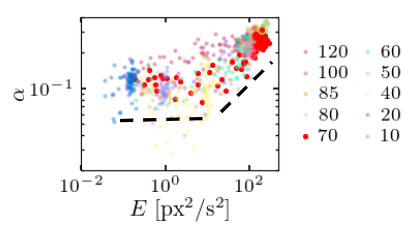
\includegraphics[width=0.5\textwidth]{figures/fig-7-v1.png}
% \caption[]{Giant number fluctuations magnitudes $\alpha$ as a function of simultaneous flow energy $E$ at concentrations 10 n$_0$ to 120 n$_0$.}
% \label{fig:7}
% \end{center}
% \end{figure}
%
% \textit{Discussion--}In dense bacterial suspensions, the close correlation between flow strength and number fluctuation magnitude, evidenced by our measurements above, suggest that the swimming-induced flow drives the evolution of concentration profile and results in the giant number fluctuations. And we have since deduced that, the difference between the plateau concentrations of $\alpha$ and spatial correlation lengths is attributed to the abrupt increase of flow energy from 40 n$_0$ to 70 n$n_0$. However, such explanation is not sufficient to understand the gradual increase of $\alpha$ from 10 n$_0$ to 30 n$_0$, where the flow energy remains nearly a constant, near 0. To find out the relation between $\alpha$ and flow energy $E$ at all concentrations, we put all the ($\alpha$, $E$) pairs extracted from evolution data on a scatter plot (see Fig.~\ref{fig:7}). All the data points constitute roughly two regimes: a nearly flat low energy regime and a fast increasing high energy regime. That the low energy regime is almost flat suggests that, when energy is low, it is no longer determining the magnitude of number fluctuations. Therefore, since the gradual increase of $\alpha$ with concentration happens in this low energy regime, we expect that it should be attributed to other mechanisms. We highlight the data points for 70 n$_0$ in the plot, and have a remarkable observation: even in a dense bacterial suspension, where strong flow will eventually develop, when flow energy is low, $\alpha$ remains flat. Only until a critical energy is reached, will $\alpha$ shoot up with flow energy. So it is likely that, even in dense suspensions, before strong flow builds up, another mechanism is dominating the giant number fluctuations.
%
% \textcolor{red}{This mechanism could be dynamic clustering, which is often observed in synthetic active particle suspensions
%  \cite{PhysRevLett.108.268303, Palacci2013, PhysRevLett.123.208002}. In such systems, the motility of particles are not sufficient to induce large scale strong flows. Yet, due to their motility and rotational diffusivity (or tumbling), the particles are constantly merging into clusters and breaking apart, which are sufficient to constitute giant number fluctuations.}
%
% Though the number fluctuation in dilute, low energy regime is posing an equally interesting and rich system to study, it is out of the scope of this paper without further convincing observations. We speculate a possible scenario that could account for the gradual increase of $\alpha$, and hope to stimulate further study on this matter.
%
%
%
% \textit{Conclusion--}We have systematically measured the concentration dependence, evolution and detailed flow-concentration coupling and revealed that the motility induced large scale flow drives the giant number fluctuations and determines their strength in dense bacterial suspensions. \textcolor{red}{We also find that reduction in dimensionality lowers the magnitude of giant number fluctuations, contradicting theoretical predictions.} Lastly, we show that the gradual increase of the magnitude of number fluctuations in dilute bacterial suspensions is not accounted for by the large scale flow strength, and should be attrbute to other mechanisms.
%
% We acknowledge the support from NSF and DARPA.

\bibliographystyle{apsrev4-2}
\bibliography{correlation}



\end{document}
